\chapter{Introduction}

The history of the formation of stars is a key topic in the understanding of galaxies since it determines most of the physical processes of the initial stages and evolution of these building blocks of our Universe. Understanding the way stars form allows us to comprehend many physical properties of their host galaxies thus providing a useful framework on which to build a more elaborate theory of their subsequent evolution. We might have good ideas and some general agreement in the basics of formation of stars in galaxies, but our observational limitations don't allow us to say much about distant objects which we need to make a more elaborate and complete theory. In principle, we can't assume that all the stars have the same formation history in every galaxy and for every epoch of the Universe. The gas clouds that form stars might or might not create the same mixture of stars in every stellar system so it is important to see under what conditions we could assume a general trend and what implications in our observations this may have.

For galaxies that are far away, it is impossible to make star counts with our current technology, for this reason, their mass-to-light-ratio $\Upsilon$ (given by their stellar populations) provides a simple constraint on their number of stars per unit mass given by the initial mass function  (IMF, which is a very fundamental and important quantity in the study of stellar systems because it constraints the physics of star formation but also because it allows us to infer stellar masses through observed luminosities.) as discussed by Russell J. Smith \& John R. Lucey, \citeyear{Reference7}. Everything we know from galaxy evolution is implicitly assuming an explicit form of the IMF, with very little variations since it is the method we use to connect evolutionary sequences, this of course, given the fact that if every galaxy had its own IMF then it would be too difficult to study their evolution because of the lack of any knowledge about their history. We have some observational information about IMF in galaxies, in the case of spiral galaxies for example, the most commonly used IMFs are Chabrier or Kroupa which are decently constrained given the facilities of our observations in our own galaxy. Also, bulges appear to have heavier IMFs than disks as mentioned by (Brewer et. al \citeyear{Reference16}), but our current understanding of this topic is still quite far from being satisfactory.

Although these naive assumptions given by our limited observational evidence might not be too far from reality, we must note that when we study more complex and dense systems like the brightest cluster galaxies (BCG) in galaxy clusters or giant elliptical galaxies in general, constraining the IMF via $\textrm{M}_{\star}/\textrm{L}$ might be way more complex and poses a greater challenge since masses are more difficult to establish for dynamically-hot systems like them. Measuring $\Upsilon$ in these systems is not a truly accurate constraint on the IMF since we may have different stellar formation histories than the ones associated with galaxies that are being formed now. These objects have a very old origin (although their build up and morphological formation is recent) because their stellar populations are old and they correspond to the highest density peak, so it is difficult to relate their stellar populations accurately.

This general view shows that in the context of the evolution of galaxies, there are many things that come together at the very heart of cosmology but also in the context of the stellar astrophysics and they need to be consistent with each other. Addressing this problem is complex for many reasons, one of them is that these systems have a strong dependency on their non-baryonic matter content which affects the mass-to-light-ratio determination. This dark matter contribution accounts for most of the dynamical mass of galaxies and it's the dominant contribution in most of their spacial scales, specially in the outer regions. The problem would be much easier to study if we only had the stellar mass because the light measurements would be enough to constrain the stellar populations, their evolution and their mass distribution. 

Being able to calculate the percentage of dark matter allow us to define the IMF more precisely. So we want to see what fraction of the surface density is given by stars and what are the spatial scales in which DM becomes the dominant contribution to the enclosed mass. DM halos seem to have a diluted profile in comparison to the stellar content of galaxies (Navarro Frenk White, \citeyear{Reference17}) so there is a region near the center of these massive systems in which the stellar mass is the dominant contribution. This implies that accurate measurements of their luminosity could give precise determinations of their mass to light ratio thus giving us some knowledge of their IMFs.

Various techniques have been developed to try to understand the stellar populations that form these massive systems. One of them is by using gravitational lensing (Treu et. al. \citeyear{Reference1})  of  background galaxies. Modelling the lensing configuration on a BCG provides a useful method to determine stellar and dark matter mass contribution in elliptical galaxies, since it is difficult to constraint the IMF via $\textrm{M}_{\star}/\text{L}$ as mentioned before. Finding strong lensing in these systems can also give us information about the location of the mass center of the cluster through the lensing they produce. We usually assume that the centre of galaxy clusters lies in the BCGs (George et. al. \citeyear{Reference18}) but the real position of the centre in galaxy clusters is still an unsolved problem (Harvey et. al, \citeyear{Reference13}). 

In this project we work with galaxy clusters that might be in the right range to search for gravitational lensing in the inner regions. We use deep data from CFHT that allows us to search for interesting targets and probe the relevant spacial scales. We focus on the brightest cluster galaxy since it is a very massive system that could lens background objects and because photometry measurements can be made very accurately on them in comparison with their neighbouring galaxies. Although removing the BCG with theoretical models is quite difficult, it is still a good target to look at. 

Several recent studies have investigated whether the IMF systematically varies with galaxy mass, in particular among elliptical galaxies. These analyses are mostly based on two independent approaches. The first is an indirect method, where galaxy stellar masses are determined from stellar population synthesis models that actually do not resolve the IMF: the IMF is adjusted until the population-synthesis mass-to-light ratio matches independent constraints from dynamics and/or lensing. The second, direct method uses features in galaxy spectra that are particularly sensitive to the presence of, e.g., dwarf stars to determine the IMF directly from spectroscopic observations. Both approaches come to the same result: although there is significant galaxy to galaxy scatter, lower mass early-type galaxies (with dispersions $\sigma \approx 200$ km/s) seem to be roughly consistent with a Milky-Way type IMF (e.g. a Kroupa or Chabrier IMF). In high-dispersion elliptical galaxies, however, stellar mass-to-light ratios are about a factor of 2 times higher than expected from a Kroupa IMF. Direct studies specifically indicate that the IMF in massive galaxies seems to be more dwarf dominated than in the Milky-Way (and can be described, e.g., by a Salpeter IMF).

It's difficult to see how much of the faint stars contribute to the mass of the system. We only see the new bright ones

One way could be through dynamics, another could be through gravitational lensing. If we take different IMFs, how sensitive is the matter content to the choice of IMF?. Smaller the dark matter contribution, the smaller the overall error you make since light is easier to constraint and thus the IMF. Strong lensing measures exactly the enclosed mass so we need to know how much of its contribution we need to subtract, the less we have to subtract, the better for the determination of the IMF. If the effect of the IMF is very subtle in the mass vs radius plot, then we would need to know the dark matter distribution very well, but if the effect of the IMF is not very subtle, the less you need to know about the dark matter distribution. A recent study of a BCG mentions the relevance of this spatial scale, at very small radii stars dominate the lensing mass, so that lensing provides a direct probe of the stellar mass-to-light ratio, with only small corrections needed for dark matter (Russell Smith and John R. Lucey \citeyear{Reference7}) 

That's why the IMF is relevant, because it allows to see how much it moves up and down. If you look at a galaxy, why is it not possible to get the mass to light ratio? This is because the dark matter is more diluted than stellar light so the mass follows light behaviour is not valid and a well understood theory of the dark matter halos has to be taken into account, NFW (Navarro, Frenk \& White, \citeyear{Reference17}) provided a very consistent model for dark matter halos using N-body simulations so we can relate the lensing of the halos given this NFW density profile and putting special attention in the spacial scales on which the dark matter is relevant and where it starts to be the dominant contribution of the system and thus the lensing.

For stars, measurements of the luminosity function can be used to derive the Initial Mass Function (IMF). For galaxies, this is more difficult because Mass to light ratio (M/L) of the stellar population depends upon the star formation history of the galaxy. Bulges have heavier IMFs than disks.

The $\text{M}_{\star}/L$ depends on galaxy type, but due to the lack of multi-wavelength photometry, it is often assumed that all cluster galaxies are composed of the same stellar population. If one assumes an old stellar population (and therefore a high $\text{M}_{\star}/L$), the mass of the late-type galaxies (and thus the cluster as a whole) is over-estimated. \citeyear{Reference2}.

Galaxy clusters contain a population of stars gravitationally unbound to individual galaxies, yet still bound to the clusters overall gravitational potential, created by the stripping of stars from galaxies during interactions and mergers.

Mass-to-light ratios of early-type galaxies are of particular interest to understand the tilt of the fundamental plane. Virial relations imply that the effective surface brightness $I_{\text{eff}}$, the effective radius $r_{\text{eff}}$ and the central velocity dispersion $\sigma_{0}$ in hot stellar systems are not independent of each other. This is revealed by the fundamental plane of early type galaxies.

Several recent studies have presented evidence for ``heavyweight" IMFs in giant ellipticals, with a mass-to-light-ratio twice that of a Milky Way like IMF.    
   
\begin{figure}[H]
\centering
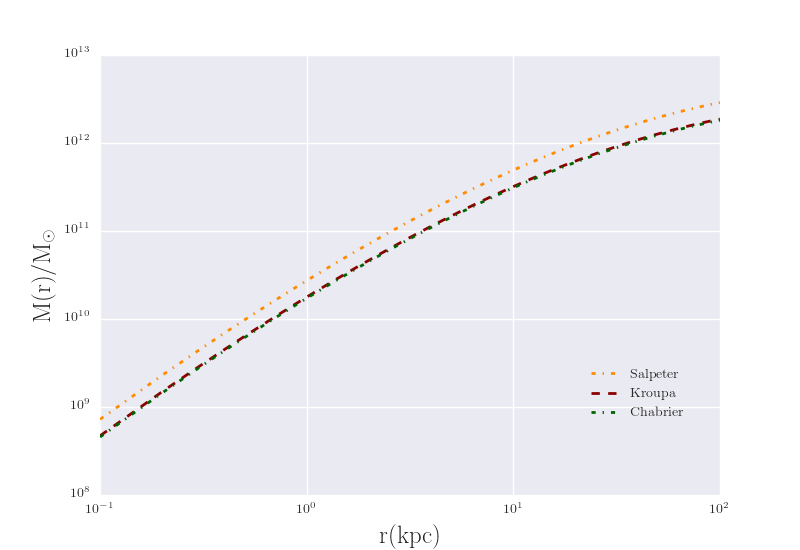
\includegraphics[width=12cm]{images/Enclosed_Mass_IMFs.png}
\caption[Enclosed mass for different IMFs in a galaxy]{Enclosed mass for different IMFs in a galaxy of $M_{200}\approx 10^{12} M_{\odot}$}
\end{figure}   